\documentclass[class=article, crop=false]{standalone}
\usepackage[subpreambles=true]{standalone}
\usepackage{import}
\usepackage{ebproof}
\usepackage[utf8]{inputenc}
\usepackage{tikz}
\usepackage{hyperref}
\usepackage{amsmath}
\usepackage{amssymb}
\usepackage{listings}
\usepackage{verbatim}
\usepackage{a4wide}
\usepackage{float}
\usepackage[justification=centering]{caption}

\lstdefinelanguage{efflang}
{
    % list of keywords
    morekeywords={
        let,
        perform,
        continue,
        val,
        effect,
        in,
        if, then, else,
        with, handle, handler,
        finally,
        match
    },
    sensitive=false,
    morecomment=[s]{(*}{*)},
    morestring=[b]"
}

% Define Colors
\usepackage{color}
\definecolor{eclipseBlue}{RGB}{42,0.0,255}
\definecolor{eclipseGreen}{RGB}{63,127,95}
\definecolor{eclipsePurple}{RGB}{127,0,85}
\definecolor{bg}{RGB}{248,248,248}

\lstset{
    language={efflang},
    basicstyle=\small\ttfamily, % Global Code Style
    captionpos=b, % Position of the Caption (t for top, b for bottom)
    extendedchars=true, % Allows 256 instead of 128 ASCII characters
    tabsize=2, % number of spaces indented when discovering a tab 
    columns=fixed, % make all characters equal width
    keepspaces=true, % does not ignore spaces to fit width, convert tabs to spaces
    showstringspaces=false, % lets spaces in strings appear as real spaces
    breaklines=true, % wrap lines if they don't fit
    %frame=trbl, % draw a frame at the top, right, left and bottom of the listing
    %frameround=tttt, % make the frame round at all four corners
    framesep=4pt, % quarter circle size of the round corners
    numbers=left, % show line numbers at the left
    numberstyle=\tiny\ttfamily, % style of the line numbers
    commentstyle=\color{eclipseGreen}, % style of comments
    keywordstyle=\color{eclipsePurple}, % style of keywords
    stringstyle=\color{eclipseBlue}, % style of strings
    xleftmargin=.05\textwidth,
    framexleftmargin=17pt,
    backgroundcolor=\color{bg}
    %xrightmargin=.2\textwidth
}

\renewcommand{\leadsto}{\rightsquigarrow}

\newcommand{\effFalse}{\mathbf{false}}
\newcommand{\effTrue}{\mathbf{true}}
\newcommand{\effSucc}{\mathbf{succ}\ }
\newcommand{\effFun}{\mathbf{fun}\ }
\newcommand{\effZero}{\mathbf{0}}
\newcommand{\effHandler}{\mathbf{handler}\ }
\newcommand{\effVal}{\mathbf{val}\ }
\newcommand{\effBar}{\ \textbf{\textbar}\ }
\newcommand{\effWith}{\ \mathbf{with}\ }
\newcommand{\effHandle}{\ \mathbf{handle}\ }
\newcommand{\effIf}{\mathbf{if}\ }
\newcommand{\effThen}{\ \mathbf{then}\ }
\newcommand{\effElse}{\ \mathbf{else}\ }
\newcommand{\effAbsurd}{\mathbf{absurd}\ }
\newcommand{\effMatch}{\mathbf{match}\ }
\newcommand{\effLet}{\mathbf{let}\ }
\newcommand{\effIn}{\ \mathbf{in}\ }
\newcommand{\effRec}{\mathbf{rec}\ }
\newcommand{\tto}{\twoheadrightarrow}

\begin{document}

This chapter of my dissertation contains a discussion on the theoretical background
of the project. It also describes other work which had to be
undertaken before I wrote any code, contains the starting point of my project
and the development methodology I used to carry out the work.

% \section{Computational effects}

% There are two types of programs: pure and effectful (or impure). Pure programs are ones that are independent from the environment and effectful programs are the ones that \emph{do} something in the
% sense that they interact with their environment. Another way of defining pure functions is: given the definition of the function and its arguments, its result is uniquely determined.

% Programs invoking computational effects such as nondeterminism, probabilistic nondeterminism, exceptions, interactive input/output or side effects all constitute as effectful. This is obvious for
% interactive input/output, nondeterminism and side-effects as these obviously interact with the environment. Exceptions are a bit awkward in the sense that throwing them is pure but catching them is
% not (consider catching an exception that is thrown due to an out-of-memory error; catching this exception would mean that we interact with the environment in an implicit way).

% Reasoning about pure programs is easy, as pure computations (partial functions) are well understood. However, most programs must \emph{do} something with the real world (write to a file, 
% read from a network socket, handle errors, generate random numbers, etc.) and perform effects to be useful.
% Hence, to be able to reason about our programs we must properly understand the properties of these effects, how they work, how they interact and what rules apply to them. To do this, we try to model
% them in a framework that was always know to work: mathematics.

\section{Eff by example}

Eff is a programming language based on algebraic effect handlers.
Essentially, it is a pure subset of OCaml \cite{ocaml-website} extended with a few extra
keywords which implement effects and effect handlers: \verb|effect|,
\verb|perform|, \verb|handler|, \verb|continue|, \verb|with-handle| and \verb|finally|.
What follows is a brief introduction of these features by using the
unmissable Hello World example.

\subsection{Effects}

Effects lie in the heart of Eff (hence the name). A programmer can define
effects using the \verb|effect| keyword, the effect's name (effect names must
be capitalized just like OCaml variant tags) and its type. An effect definition
can be seen on \autoref{effect-perform-keywords}. Effects always have a type
of $A \tto B$ for some types $A$ and $B$.

\begin{figure}[hbt!]
  \lstinputlisting[caption={Printing can be thought of as an effect with an argument of type
  string and a result of type unit.}, label=effect-perform-keywords]{../code_examples/first_program.eff}
\end{figure}

\subsection{Performing effects}

Effects behave a bit like functions as we could see from their types above.
Once an effect of type $A \to B$ is defined we can invoke it
using the \verb|perform| keyword and by providing an argument of type $A$.
The type of the resulting expression is $B$.

The \verb|perform| keyword is similar to \verb|raise| in OCaml or to \verb|throw|
in Java in that when we perform an effect the control will be given to an effect
handler (this would be an exception handler in OCaml or Java) or the program
will terminate with an exception if no handler can handle the effect.

Don't be confused by how an effect is constructed. Effects are not values in
the Eff language. That is, \verb|Print "Hello World"| would be meaningless in
itself, just like the exception \verb|Failure "hd"| would be meaningless in OCaml
if we did not raise it. The situation is similar here but effects are \emph{performed} and not raised.

\subsection{Handlers}

Handlers give meaning to effects: this is what programmers can use to specify
what they mean by an effect, such as \verb|Print| in \autoref{effect-perform-keywords}.
An effect can be declared without a handler, but when performed, can only cause a program 
to terminate with an exception.

Handlers are first-class citizens (i.e., values) in Eff. One can define them with the
\verb|handler| keyword by specifying \emph{rules}.
An example can be seen on \autoref{handler-keyword}.


\lstinputlisting[caption={A handler definition consisting of 2 cases: a value case and an effect case.}, label=handler-keyword]{../code_examples/print_handler.eff}

% TODO:  and a finally rule. The effect rule first resumes the rest of the program to obtain its result and its output. ``Printing'' out \texttt{message} is simulated by string concatenation; we prepend \texttt{message} to the output of the rest of the program.

To complete our Hello World example we must be able to \emph{apply} this handler. This is done
using a \emph{with-handle block} as illustrated on \autoref{hello-world}.

\lstinputlisting[caption={The Hello World example in Eff. The code above evaluates to the pair \texttt{((), "Hello World!")}.}, label=hello-world]{../code_examples/hello_world.eff}
As handlers are values, they have their own type of the form $A \Rightarrow B$.
Handler types are similar to the $\to$ function types but they work on computations
rather than on values. The handler on \autoref{hello-world} is of type \verb|unit => unit * string|
as it transforms a computation of type \verb|unit| to one of type \verb|unit * string|. 

There are various aspects of the code that can be strange on the first sight. The first
is the rules involved in the declaration.

\subsubsection{Handler rules}

One can use three kinds of rules in a handler: a \emph{value rule}, an \emph{effect rule} or
a \emph{finally rule}.\footnote{TODO: I should say \emph{case} rather than \emph{rule}. The authors use case and I noticed it
only when I re-read parts of the publication. Later I use case to mean rule. They are the same.}

A value rule has the form $x \to c$. This is a rule that describes how to handle the
\emph{return value} of a computation.
It takes the return value of a computation enclosed by a with-handle block, binds it to the
identifier $x$ and performs the computation $c$.
In \autoref{handler-keyword} we are simply saying that if the computation handled by this
handler has finished computing without invoking any effects, then we are returning a pair containing
the result of the computation and the empty string (this reflects that nothing was printed).

An effect rule is a generalisation of SML's \cite{milner1997definition} \verb|handle|. It differs from it in
that it also receives the \emph{continuation} (\verb|k| above) of the computation enclosed
by the with-handle block handling the effect. Such a continuation can be \emph{resumed} with
the \verb|continue| keyword. Note that when an effect of type $\alpha \to \beta$ is handled,
we get \emph{read access} to its argument of type $\alpha$ and we can resume its continuation if we provide
the continuation with a value of type $\beta$ it expects (this is why we resume the continuation
by giving it a \verb|()| value in \autoref{handler-keyword}---\verb|Print| is of type $string \to unit$).

Finally rules are just syntactic sugar for let wrappers around with-handle blocks.
That is, $\textbf{finally } r \to f$ does the same as $\textbf{let } r \leftarrow \textbf{with } v \textbf{ handle } c \textbf{ in } f$.
Finally rules were introduced to avoid having to use such inconvenient let wrappers \cite{bauer2015programming}.

A handler can have any number of effect rules (even zero) but only at most one finally rule and at most one value rule.
Value rules and finally rules are optional. When they are avoided they are assumed to be identities (i.e.,
\verb|x -> x| or \verb|finally x -> x| respectively).

% \subsection{Advantages}

% \subsubsection{OOP and functional style}

% We can think about effect signatures as interfaces and handlers as implementations of these interfaces.
% A \verb|with h handle c| block is then an ``instantiation'' of effect implementations.

% We see that programming with effect handlers puts us between the object-oriented and functional styles and gives us more opportunities to re-use existing pieces of code (see next code example).

% \subsubsection{Direct style}

% The following example shows an implementation of the state monad (borrowed from the official Eff website \cite{eff-website}):
% \begin{verbatim}
% effect Get: int
% effect Set: int -> unit

% let monad_state initial = handler
%   | y -> (fun s -> (y, s))
%   | effect Get k -> (fun s -> (continue k s) s)
%   | effect (Set s') k -> (fun _ -> (continue k ()) s')
%   | finally f -> f initial
% ;;

% let double_and_add_ten () =
%   let x = perform Get in
%   perform (Set (2 * x));
%   perform Get + 10
% ;;

% with monad_state 30 handle
%   double_and_add_ten ()
% ;;
% \end{verbatim}

% Note how the function \verb|double_and_add_ten| is written in a direct style. As mentioned above, the programmer does not have to 
% be aware of the implementations of the effects (indeed, we see that the ``internal'' representation of state uses functions). 
% This function illustrates how handlers increase the modularity of our programs (we could use the function in the context of other handlers 
% and perhaps get some other result).

% \subsubsection{Composition}

% Monads are frequently used as a way to simulate effectful computations in programming languages like Haskell. 
% However, combining different kinds of effects in these languages can be non-trivial and 
% tiresome sometimes. Haskell uses monad stacks and monad transformers to get around this. [TODO: someone might not know what this is]

% In Eff, combining effects and their handlers arises naturally. Handlers can be written for any set of effects and handlers can be combined 
% with nesting \verb|with ... handle| blocks.

% [TODO: I need two code examples here to justify the claims above and show that \verb|with ... handle| is more convenient. One in Haskell with monad transformers and one in Eff with two nested handlers.]

% \subsubsection{Criticism}

% Although there are many attractive properties of effect handlers, one that is frequently quoted to be ``annoying'' is that it is very easy to write incomprehensible code via continuations.
% Continuations are not a novel concept but it is one that perhaps isn't widely known by the wider software engineering community. Hence providing the concrete implementation of effects
% can impose some extra burden on a programmer's brain.


\section{Continuations and control operators}

Although continuations came up briefly in the previous section I did not explain what they are in detail.
This section is devoted to this because continuations are playing a crucial rôle in Eff and in what follows
in this dissertation.

% Continuations were first discovered in 1964 by van Wijngaarden \cite{reynolds1993discoveries}.

\subsection{Landin's J operator and call/cc in Scheme}

TODO: Landin's J operator.\\
The mechanical evaluation of expressions \cite{landin-secd}.

\subsection{Delimited continuations}

TODO: Delimited continuations

% check this out
% https://en.wikipedia.org/wiki/Delimited_continuation



\section{Monads}

\section{The Eff core formally}

\emph{Core Eff} is described in \cite{bauer2013effect}. This section is largely based on that paper.

\subsection{Syntax}

% syntactic difference between pure expressions and possibly effectful computations
% iota?
% implementations can avoid the syntactic difference
% talk about monads here

In core Eff there is a syntactic distinction between expressions and computations.

\textbf{Note to Alan:} Here I will/want to talk about:
\begin{itemize}
  \item The syntactic difference between pure expressions and possibly effectful computations
  \item $\effVal$ is \emph{return}
  \item Haskell monads (but maybe that should go to the Type and effect system?); I have trouble introducing these; I don't have a grip on them; I need a ``story''.
  \item $\iota\#op$ -- the authors use this notation; I think it is very annoying, I don't see any reason why $\#op$ is a ``thing''; I think some better notation can
    make a huge difference here and can lead to a less scary more intuitive introduction; I am thinking about just using $\iota$. Any inputs here or any conventions/notations
    I should know about? Ideas?
\end{itemize}

\begin{figure}
Expressions
$$ e ::= x \mid \effTrue \mid \effFalse \mid \effZero \mid \effSucc\ e \mid () \mid \effFun\ x\ :\ A \mapsto c \mid \iota \mid h $$
Handlers
$$ h ::= \effHandler \effVal x : A \mapsto c_v  \effBar ocs $$
Operation cases
$$ ocs ::= nil \mid (e\#op\ x\ k \mapsto c \effBar ocs)$$
Computations
\begin{align*}
  c ::= \ &\effVal e \mid e_1\#op\ e_2 (y.c) \mid \effWith e \effHandle c \mid \effIf e \effThen c_1 \effElse c_2 \mid\\
        & \effAbsurd e \mid e_1\ e_2 \mid \effMatch e \effWith \effZero \mapsto c_1 \effBar \effSucc x \mapsto c_2 \mid \\
        & \effLet x = c_1 \effIn c_2 \mid \effLet \effRec f\ x : A \to C = c_1 \effIn c_2
\end{align*}
\caption{Abstract syntax of core Eff}
\label{fig:core-eff-syntax}
\end{figure}

\subsection{Semantics}

This section presents the small step operational semantics of core Eff (see \autoref{fig:small-step-semantics}). As
expressions are pure I avoid giving reduction rules for them. The spotlight is on possibly effectful computations and
on their reduction rules given by the relation $\leadsto$.

\begin{figure}
$$
\begin{prooftree}
\hypo{}
\infer1[(\textsc{If-True})]{\effIf \effTrue \effThen c_1 \effElse c_2 \leadsto c_1}
\end{prooftree}
\quad
\begin{prooftree}
  \hypo{}
  \infer1[(\textsc{If-False})]{\effIf \effFalse \effThen c_1 \effElse c_2 \leadsto c_2}
\end{prooftree}
$$

$$
\begin{prooftree}
  \hypo{}
  \infer1[(\textsc{Fun-App})]{(\effFun x \mapsto c)\ e \leadsto c[e/x]}
\end{prooftree}
\quad
\begin{prooftree}
  \hypo{}
  \infer1[(\textsc{Match-Zero})]{\effMatch \effZero \effWith \effZero \mapsto c_1 \effBar \effSucc x \mapsto c_2  \leadsto c_1}
\end{prooftree}
$$

$$
\begin{prooftree}
  \hypo{}
  \infer1[(\textsc{Match-Succ})]{\effMatch (\effSucc e) \effWith \effZero \mapsto c_1 \effBar \effSucc x \mapsto c_2  \leadsto c_2[e/x]}
\end{prooftree}
$$

$$
\begin{prooftree}
  \hypo{c_1 \leadsto c_1'}
  \infer1[(\textsc{Let-Step})]{\effLet x = c_1 \effIn c_2 \leadsto \effLet x = c_1' \effIn c_2}
\end{prooftree}
\quad
\begin{prooftree}
  \hypo{}
  \infer1[(\textsc{Let-Val})]{\effLet x = (\effVal e) \effIn c \leadsto c[e/x]}
\end{prooftree}
$$

$$
\begin{prooftree}
  \hypo{}
  \infer1[(\textsc{Let-Effect})]{\effLet x = (\iota\#op\ e\ (y.c_1)) \effIn c_2 \leadsto \iota\#op\ e\ (y.\effLet x = c_1 \effIn c_2)}
\end{prooftree}
$$

$$
\begin{prooftree}
  \hypo{}
  \infer1[(\textsc{Let-Rec})]{\effLet \effRec f\ x = c_1 \effIn c_2 \leadsto c_2[(\effFun x \mapsto \effLet \effRec f\ x = c_1 \effIn c_1)/f]}
\end{prooftree}
$$

$$
\begin{prooftree}
  \hypo{c \leadsto c'}
  \infer1[(\textsc{Handle-Step})]{\effWith e \effHandle c \leadsto \effWith e \effHandle c'}
\end{prooftree}
$$

$$
\begin{prooftree}
  \hypo{c \leadsto c'}
  \infer1[(\textsc{Handle-Val})]{\effWith (\effHandler \effVal x \mapsto c_v \effBar ocs) \effHandle (\effVal e) \leadsto c_v[e/x]}
\end{prooftree}
$$

$$
\begin{prooftree}
  \hypo{h \stackrel{\text{def}}{=} (\effHandler \effVal x \mapsto c_v \effBar ocs) \quad (\text{op}: A^\text{op} \to B^\text{op}) \in \Sigma_E}
  \infer1[(\textsc{Handle-Effect})]{\effWith h \effHandle (\iota\#op\ e (y.c)) \leadsto ocs_{\iota\#op} (e, (\effFun y : B^\text{op} \mapsto \effWith h \effHandle c))}
\end{prooftree}
$$

\caption{Small step operational semantics of core Eff}
\label{fig:small-step-semantics}
\end{figure}

The rules for if statements, function application, match statements and the rules \textsc{Handle-Step}, \textsc{Let-Step} and \textsc{Let-Rec}
are standard. The other \textsc{Let-*} and \textsc{Handle-*} rules need more explanation:
\begin{table}
  \setlength{\tabcolsep}{0.5em}
  \renewcommand{\arraystretch}{1.4}
  \begin{tabular}{l|p{10cm}}
  Rule & Comment \\
  \hline \hline
  \textsc{Let-Val} & If a computation \emph{returns} an expression $e$, it is bound to the identifier $x$ in the computation $c$. \\ \hline
  \textsc{Let-Effect} & A computation $c$ can also reduce to an effect $\iota\#op\ e\ (y.c_1)$, where $e$ is the argument of the effect
    constructor and $(y.\ c_1)$ is a delimited continuation representing the program point $c$'s execution was stopped at. This delimited continuation can be
    used later to resume $c$. \\ \hline
  \textsc{Handle-Val} & If a computation in a with-handle block with handler $h$ reduces to $\effVal e$, then the
    \emph{value case} of $h$ (i.e., $\effVal x \mapsto c_v$) is invoked by substituting $e$ for $x$ in $c_v$. \\ \hline
  \textsc{Handle-Effect} & This rule tells us how to look up the \emph{closest matching handler} if a computation reduces to an effect.
    If no such handler exists then the program terminates with an exception. The recursive definition of $ocs_{\iota\#op}$ describes how
    to look up a \emph{matching case} in a handler. Note how a \emph{new} continuation $(y.\kappa\ y)$ is created from $\kappa$ when we reach $nil$, i.e.,
    when no case matches the effect in question.
  \end{tabular}
  \caption{Explanation of the Eff specific rules of the small step semantics}
  \label{tab:rule-explanation}
\end{table}
The definition of $ocs_{\iota\#op}$ is as follows:
\begin{align}
  nil_{\iota\#op} (e, \kappa) = \iota\#op\ e\ (y.\kappa\ y) \\
  (\iota'\#op'\ x\ k \mapsto c \effBar ocs)_{\iota\#op}(e, \kappa) = \begin{cases}
    c[e/x, \kappa/k] & \text{if }\iota\#op = \iota'\#op' \\
    ocs_{\iota\#op(e,\kappa)} & \text{otherwise}
  \end{cases}
\end{align}

\subsection{Type checking}

\begin{figure}
  $$
  \begin{prooftree}
    \hypo{x : A \in \Gamma}
    \infer1[T-Var]{\Gamma \vdash_e x : A}
  \end{prooftree}
  $$
  $$
  \begin{prooftree}
    \hypo{\Gamma \vdash_e e_1 : A}
    \hypo{\Gamma \vdash_e e_2 : B}
    \infer2[T-Pair]{\Gamma \vdash_e (e_1, e_2) : A * B}
  \end{prooftree}
  $$
  \caption{Type checking rules for Eff expressions}
  \label{fig:type-checking-expressions}
\end{figure}

\begin{figure}
  \caption{Type checking rules for Eff computations}
  \label{fig:type-checking-computations}
\end{figure}

\section{Virtual machines}

\subsection{CEK machines}

TODO: CEK machines

\subsection{The SECD machine}

TODO: SECD machines

\begin{itemize}
  \item Landin' machine
  \item Lower level than CEK machine
  \item Can implement continuations with it
  \item Dump is important
  \item Cite \cite{landin-secd}
\end{itemize}

\section{Software engineering}

\subsection{Licensing}

It is important to mention that the project fulfills licensing criteria. The dependencies of this project are
listed below with their licenses:
\begin{itemize}
\item The OCaml toplevel, version 4.06.0, GNU Lesser General Public License (LGPL) version 2.1
\item \emph{menhir} parser generator, version 20190924, GNU Library General Public License version 2
\item \emph{Alcotest}, version 0.8.5, ISC license
\item OPAM (OCaml Package Manager), version 2.0.4, GNU Lesser General Public License (LGPL) version 2.1
\item \emph{Core} standard library by Jane Street, v0.11.3, MIT license
\end{itemize}
To the best of my knowledge these licenses allow the way I am using the software mentioned above.

\subsection{Starting point}

The starting point of my project didn't change since the writing of the project proposal [TODO: ref. appendix here]:
\begin{itemize}
  % knowledge backround
  \item I read briefly about Eff and algebraic effect handlers before starting my project.
  \item I used SML and OCaml before to implement simple interpreters for toy programming languages
    and to experiment with functional programming. This is my first big project where I use functional programming.
  \item I also had a look at the OCaml ecosystem to check if it has a stable build system, if testing frameworks are available
    and whether lexer and parser generators exist.
  \item I had basic familiarity with utility tools such as version control, various IDEs and Unix-like command line interfaces.
\end{itemize}

\subsection{Requirements analysis}

TODO

% a lot of knowledge needed to be acquired
% CEK interpreter has 2 goals: one to test my understanding and the other to give a baseline

\subsection{Development methodology}

I chose \emph{test-driven development} (TDD) \cite{beck2003test} as my project's software development methodology.
The essence of TDD is that programmers work in quick iterative cycles whereby they write failing tests first and then
implement the next feature that makes the failing test cases pass.
Always having an \emph{automated} test suite at hand avoids trial and error testing which would be both error prone and
time consuming.
The reasons for choosing this methodology was three-fold.

Firstly, the nature of my project is such that the
correctness of any code written is very well-defined as I can take the semantics of Eff
as a baseline and given a piece of code it is always possible to tell whether it is
interpreted correctly or not. This makes it possible to write tests upfront.

Second, the structure of my project imposed an order on the parts to be delivered. This is
because every module of my project (apart from the front end) depends on a previous one (see
\autoref{fig:project-structure}) and hence on its
correctness. As TDD is also known as 
``a way of managing fear during programming'' it came handy that I could write code with confidence knowing
that the code I have written before is tested. Other advantages were the ability to notice
quickly if a code change broke some already implemented feature and the ability to refactor
code with confidence (which I had to do frequently---from summer internships I knew that my coding style
is such that this will be unavoidable if I want to work with a maintainable codebase).

Third, my success criterion was a correct working implementation of a compiler so tests were
crucial to demonstrate that success criteria were fulfilled.

\begin{figure}[htb]
  \centering
  \resizebox{0.85\textwidth}{!}{
  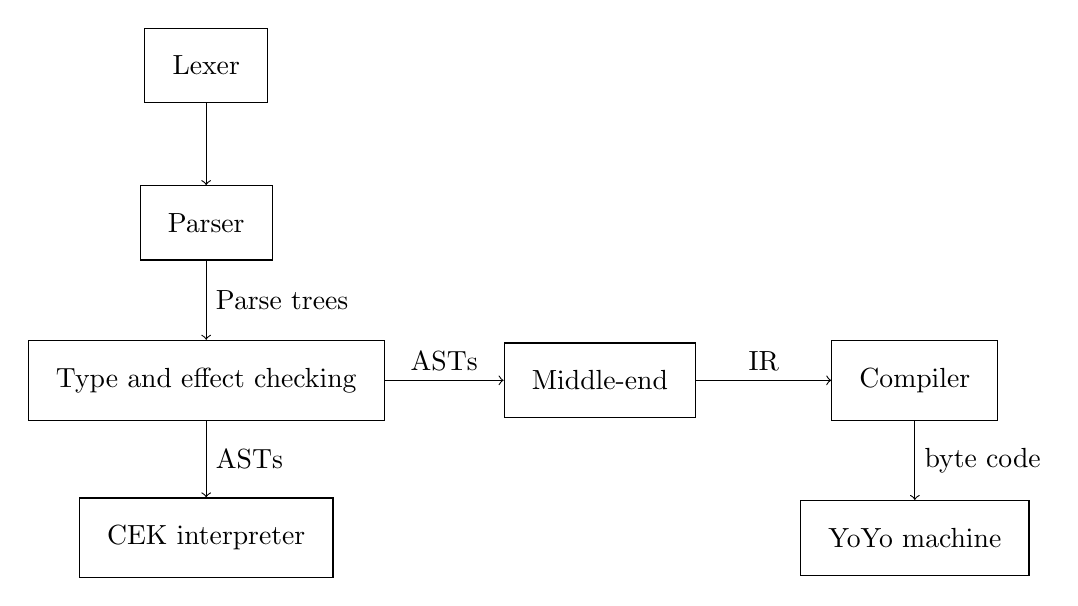
\begin{tikzpicture}
    \node[draw,inner sep=10pt] (LEX) at (0,6) {Lexer};
    \node[draw,inner sep=10pt] (PAR) at (0,4) {Parser};
    \node[draw,inner sep=10pt] (TYPE) at (0,2) {Type and effect checking};
    \node[draw,inner sep=10pt] (MID) at (5, 2) {Middle-end};
    \node[draw,inner sep=10pt] (COMP) at (9,2) {Compiler};
    \node[draw,inner sep=10pt] (CEK) at (0,0) {CEK interpreter};
    \node[draw,inner sep=10pt] (YOYO) at (9,0) {YoYo machine};
    
    \draw[->] (LEX) -- (PAR);
    \draw[->] (PAR) -- (TYPE) node[midway, right] {Parse trees};
    \draw[->] (TYPE) -- (CEK) node[midway, right] {ASTs};
    \draw[->] (TYPE) -- (MID) node[midway, above] {ASTs};
    \draw[->] (MID) -- (COMP) node[midway, above] {IR};
    \draw[->] (COMP) -- (YOYO) node[midway, right] {byte code};
  \end{tikzpicture}}
  \caption{Structure of the project}
  \label{fig:project-structure}
\end{figure}

\section{Summary}
This section summed up the theory background which was needed to complete this dissertation.
It also shows the preparation I undertook in the software engineering aspects of the project.

\begin{itemize}
  \item I briefly introduced the programming language Eff and talked about its characteristic features. I showed
    code examples demonstrating how handlers can be used in a direct style and how they support modularity and
    code reuse in functional programs.
  \item I explained the idea of a continuation, how it represents an arbitrary program point in the
    execution of a program and how it allows advanced control flow to be implemented.
  \item I gave an overview of control operators (including Landin's J operator), why they were studied in the 
    early days of programming languages and their rôle in the development of different virtual machines.
  \item I talked about the small-step operational semantics of core Eff as well as a type and effect
    system one can use with it. We saw that with-handle blocks compose naturally as opposed to monads in Haskell
    where the use of monad transformers is unnatural.
  \item I showed two examples of virtual machines which can implement the structured \emph{non-local
    flow of control} continuations make possible. The key challenge these machines solve is that
    they can \emph{save and restore} execution contexts in an appropriate way whenever non-local control flow occurs.

    A CEK machine does this by keeping a stack of continuations (K), while the SECD machine does this by using
    a so-called dump (D). The importance of these machines will become clearer in the Implementation section where I describe the
    Yoyo virtual machine for Eff which has similarities with both of these virtual machines.
  \item I stated my starting point, the timeline of my project and discussed the development methodology used
    to write the code and the testing strategy to assess its correctness.
\end{itemize}


\begin{comment}
\subsection{Eff}

This subsection gives a short introduction to Eff with some code examples.
The precise syntax and semantics of the language will be defined later,
we aim for an intuitive introduction here.

\subsubsection{Effects}

There is an important distinction between syntactic and semantic elements in the language. Effect declarations belong to syntax.

An effect in Eff is declared using the \verb|effect| keyword together with a type signature which forms the effect signature. One would define a \verb|Print| effect for printing strings as follows:



This tells us two things. To invoke the \verb|Print| effect we must provide a string as an argument and what we get back is something of type \verb|unit| after the effect is performed. We get to know no extra information about \verb|Print|.

Now that we have a \verb|Print| effect we can write down the mandatory Hello World example:
\begin{verbatim}
perform (Print "Hello World!")
\end{verbatim}

The \verb|perform| keyword is used to perform already declared effects. However, if we think about it, this piece of code still does
not make any sense as we don't know how to interpret \verb|Print "Hello World!"|.

\subsubsection{Handlers}

Handlers are used to assign meaning to effects. A handler is just a list of rules. A rule can be of three different types: a value rule, an effect rule or a finally rule.

\textbf{Value and effect rules}

The following handler provides an interpretation for the \verb|Print| effect. This handler converts the result of a computation to a 2-tuple where the first element is the original result and the second
element is a concatenation of the strings from all the \verb|Print| effects from the computation.

We use the value rule \verb|v -> (v, "")| to say what happens ``by default''. If the computation didn't print anything then we simply say that it printed the empty string.

\begin{verbatim}
let collect = handler
| v -> (v, "")
| effect (Print str) k ->
    (* Find out what the rest of the computation would print out *)
    let (result, s) = continue k () in
    (* Prefix the string printed by the rest of the computation 
       with `str` from this effect *)
    (result, str ^ s)
\end{verbatim}

The effect rule is a bit more involved. Effect rules have the form \verb|effect E(args) k| where \verb|k| is always bound to the ``rest of the computation'' which we call a continuation (and by convention
usually use the letter $k$ or $\kappa$ to denote it). The arguments of the effect \verb|E| are bound to \verb|args| via pattern matching. In the example above we first resume the computation by resuming the
computation via \verb|continue|. After we find out what the rest of the computation would print out, we prepend our current string to it.

Note that when we handle an effect of type $\alpha \to \beta$ we get a continuation of type $\beta \to \gamma$ where $\gamma$ is the type of the computation being enclosed in a \verb|with ... handle| block.

Value rules can be omitted in handler definitions, in which case they are assumed to be identities.

\textbf{Finally rules}

Finally rules are just syntactic sugar for \verb|let| wrappers around \verb|with ... handle| statements that act on the result of a handled computation, i.e.,
\begin{verbatim}
let h = handler
    | finally x -> x + x
in 
    with h handle c
\end{verbatim}
would be syntactic sugar for
\begin{verbatim}
let x = with h handle c in x + x.
\end{verbatim}

I would like to point out that this syntax is added only for convenience as it happens many times that the same transformations must be performed after a \verb|with ... handle| block \cite{bauer2015programming}. Hence \verb|finally| here does not provide the Java-like semantics where the computation in a finally block is ``guaranteed'' to be executed.

Finally rules can be omitted in handler definitions, in which case they are assumed to be identities.

\textbf{Handler types}

Handlers handling a computation of type $\alpha$ and giving a result of type $\beta$ are given the type $\alpha \Rightarrow \beta$.
\end{comment}

\begin{comment}
\subsection{TODOs}
\begin{itemize}
\item I haven't said anything about shallow and deep handlers
\item Comparing to haskell monads/monad transformers is risky -- need to explain these
\end{itemize}

\section{Papers}
\begin{itemize}
\item Delimited control \cite{kiselyov2010delimited}
\item Eff Directly in OCaml \cite{Kiselyov_2018}
\item Very good article about CPS compilation \cite{flanagan1993essence}
\item Bauer tutorial \cite{bauer2018algebraic}
\end{itemize}
\end{comment}

\ifstandalone
\bibliography{../bibliography}{}
\bibliographystyle{plain}
\fi

\end{document}